% \chapter{Search spaces}

\newpage

Before going further with our quest for efficient RL. Let's try to understand
some properties of our setting, MDPs.


\section{The value function polytope}

The Value Function Polytope \cite{Dadashi2018} provides some great intuition
about the structure of a MDP and the dynamics of solvers. Let's take a look:
consider a two state, two action MDP.

\begin{figure}[hb!]
\centering
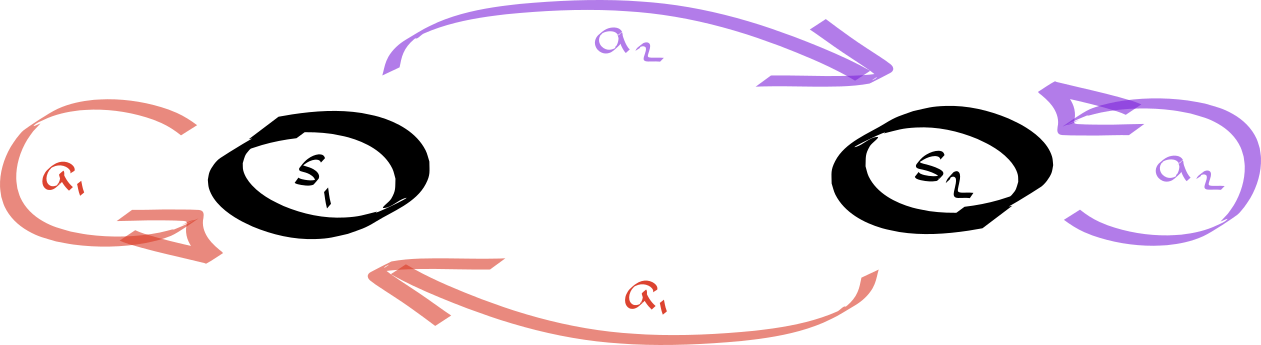
\includegraphics[width=1\textwidth,height=0.25\textheight]{../../pictures/drawings/2-state-automata.png}
\caption{The simplest possible MDP has two states and two actions. (Any simpler setting is entirely uninteresting. A single state means actions do nothing.
And a single action means all policies are the same.).}
\end{figure}

The space of possible policies is a 2D surface in a 4D space. For each state, we
can pick action 1 or action 2, with some probability, $p$.

\begin{align}
\pi &=
\begin{bmatrix}
  p(a=a_1|s=s_1) & p(a=a_2|s=s_1) \\
  p(a=a_1|s=s_2) & p(a=a_2|s=s_2)\\
\end{bmatrix} \\
&=
\begin{bmatrix}
p(a=a_1|s=s_1) & 1-p(a=a_1|s=s_1) \\
p(a=a_1|s=s_2) & 1-p(a=a_1|s=s_2)\\
\end{bmatrix}
\end{align}

Since the policies are a 2D space, we can visualise them. This square of all possible policies is not particularly interesting.

Rather, we can evaluate (calculate the expected return) each each policy (using the \eqref{eq:value-functional}).
Since there are two states, the evaluation returns a 2D vector of values, one value for each state.
We can easily visualise the value of each policy. And because the policies were a 2D structure, we see a

\begin{figure}[!hb]
\centering
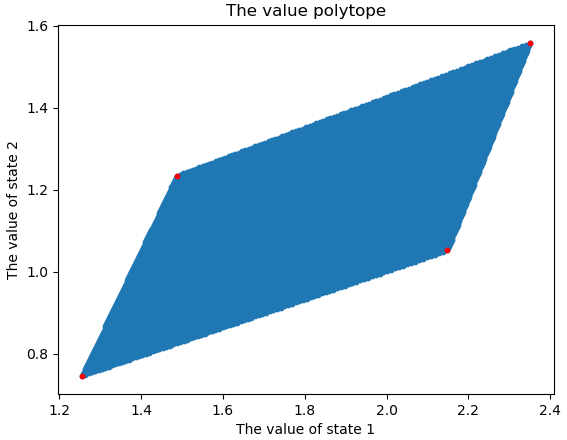
\includegraphics[width=1\textwidth,height=0.5\textheight]{../../pictures/figures/value-polytope.png}
\caption{For every policy, we can plot a dot where that value of that policy lies in 'value space'.
The red dots are deterministic policies.}
\end{figure}

\subsection{Properties of the polytope}

Dadashi et al. \cite{Dadashi2018} explored a few properties of the polytope. Sepcifically they focused on its geometry and dynamics. \footnotemark[3]

\footnotetext[3]{In \ref{polytope-extras} you can find further exploration of other properties of the value polytope.}

\subsubsection{Geometry of the polytope}

Dadashi et al. remark, the polytope gives a clear illustration of the following classic results regarding MDPs \cite{Bertsekas1996}.

\begin{itemize}
\tightlist
  \item (Dominance of $V^*$) The optimal value function $V^*$ is the unique dominating vertex of $V$;
  \item (Monotonicity) The edges of V are oriented with the positive orthant;
  \item (Continuity) The space V is connected.
\end{itemize}

{\color{red} i need to explain these!?}

% Further more, Dadashi et al show that ... Line theorem. s-deterministic policies.

\subsubsection{Dynamics on the polytope}

Furthermore, Dadashi et al. were interested in three aspects of different algorithms’ learning dynamics:

\begin{itemize}
\tightlist
  \item the path taken through the value polytope,
  \item the speed at which they traverse the polytope,
  \item and any accumulation points that occur along this path.
\end{itemize}

% Why do they care?
% How quickly do these learners traverse the polytope? Do algorithms take the shortest path? Where are the accumulation points?

They consider value iteration, policy iteration, policy gradients, entropy regularized policy gradients,
natural policy gradients and the cross entropy method.

Their results are intriguing. They show that different RL algorithms traverse the polytope in vastly different ways.
Some are not even constrined to the polytope. This left me wondering;

{\color{red}I feel like this needs more}

\begin{displayquote}
  \textit{How does a search algorithm interact with its search space to yield efficient search?}
\end{displayquote}

\section{Search spaces for RL}

We want to efficiently find the optimal policy for a given MDP. But where and how should we
search for this policy? We could search within;

\begin{itemize}
\tightlist
  \item the set of potentially optimal policies, the $|A|^{|S|}$ discrete policies,
  \item the set of all possible policies $\pi \in \mathbb R^{|S| \times |A|}: \forall s \int_a \pi(a|s) = 1$
  \item the set of possible value functions, $\mathbb R^{|S|}$, which we could then use to construct the optimal policy,
  \item Or maybe some other space.
\end{itemize}
But, which space is best? Which space allows us to find the optimal policy in the 'cheapest' manner?

Naively, we know that smaller search spaces are better. We would rather
search for our keys in a few rooms, rather than many. But added
structure (for example, an ordering) can be exploited to yield faster
search, even when there are infinitely more states to search. For example,
we might be able to order the rooms based on how recently we visited them.
This should help us retrace our steps and find our keys, rather than arbitrarily
picking rooms to search.

\subsection{Policy search}

We can search through policies. In my opinion, this feels like the most 'natural' type of search for RL.
As, after all, we are searching for the optimal \underline{policy}.

Searching through the space of policies supports a couple of modes of travel:
policy iteration jumps between deterministic policies (the verticies of our polytope).
Policy gradients takes small steps in the 'right' direction and often traverses through the center of the polytope.

\subsubsection{Policy iteration}

In our tabular setting, policy iteraction can be written as:

\begin{algorithm}
\caption{Policy iteration}
\begin{algorithmic}[1]

\Procedure{PI}{$P, r, \gamma$}
    \State $\pi = \text{init}()$
    \While{not converged}
      \State $V(\pi) =  (I - \gamma P_{\pi})^{-1} r_{\pi}$ \Comment{Evaluate policy}
      \State $\pi = \mathop{\text{argmax}}_\pi \big[r_{\pi} + \gamma P_{\pi}V(\pi) \big]$ \Comment{Greedy update}
    \EndWhile
    \State \algorithmicreturn{ $\pi$}
\EndProcedure

\end{algorithmic}
\end{algorithm}



\subsubsection{Policy gradients}

\begin{algorithm}
\caption{Policy gradients}
\begin{algorithmic}[1]

\Procedure{PG}{$P, r, \gamma, \eta$}
  \State t = 0
  \State $\pi_t = \text{init}()$
  \While{not converged}
    \State $\pi_{t+1} = \pi_t + \eta \nabla_{\pi} V(\pi)$ \Comment{Gradient update}
    \State t += 1
  \EndWhile
  \State \algorithmicreturn{ $\pi_t$}
\EndProcedure

\end{algorithmic}
\end{algorithm}


add ref

% Want to include upper / lower bounds!?

\subsection{Value search}

Let's search through possible values. But how can we ensure that our search will
converge to a value reasliable by the original MDP? We can use Bellman's
optimality operator to guide the search.

% (need to explain? why does stationarity mean optimality...?!)
Intution about why it converges!? Contraction. Banach fixed-point theorem.

% \begin{align}
% T(V) &= \mathop{\text{max}}_a \big[r + \gamma PV\big] \\
% \end{align}

\begin{algorithm}
\caption{Value iteration}
\begin{algorithmic}[1]

\Procedure{VI}{$P, r, \gamma, \eta$}
  \State t = 0
  \State $V_t = \text{init}()$
  \While{not converged}
    \State $\hat V = r + \gamma PV_t$ \Comment{Evaluate}
    \State $V_{t+1} = V_t + \eta (\hat V - V_t)$ \Comment{Average}
    \State t += 1
  \EndWhile
  \State $\pi = \mathop{\text{argmax}}_{\pi} r_{\pi} + \gamma P_{\pi}V_t$
  \State \algorithmicreturn{ $\pi$}
\EndProcedure

\end{algorithmic}
\end{algorithm}


% Want to include upper / lower bounds!? On complexity. Sample / computational!?

Observe that the value iterations are not constrained to refer to any policy,
and thus can go outside of the polytope. \cite{Dadashi2018}

{\color{red}mportant. Also, why does it go outside?!?}

We are constrained to move around by only using the Bellman optimality operator.
To move proportionally to value improvement of the best actions ...
Why is this good / bad. What dynamics can / cannot be achieved?

\begin{center}\rule{0.5\linewidth}{\linethickness}\end{center}

So there are different classes of search space: each imbued with special
structure from the Bellman equation or expected return. Each with different types of search they
support. And each with different parameter topologies.

Which spaces support efficient search for the optimal policy? Can we characterise the properties of each space?

\section{Gradient based search}

{\color{red}need a better seguae into GD?!}
Let's focus on searching with gradient descent.

\begin{align}
w_{t+1} = w_t - \eta \nabla f(w_t)
\end{align}

The dynamics of the search are dependent on the topology of a problems loss surface.
The loss surface is determined by the combination of the search space and the loss function.

\subsection{Parameterised search}

Overparam. DL. \cite{Arora2018}

\begin{align}
&\mathop{\text{max}}_V \mathop{\mathbb E}_{s\sim D} V(s) \\
&\mathop{\text{max}}_{\pi} \mathop{\mathbb E}_{s\sim D}V^{\pi}(s) \\
&\mathop{\text{max}}_{\theta} \mathop{\mathbb E}_{s\sim D} V_{\theta}(s)\label{eq:deepQ}\\
&\mathop{\text{max}}_{\theta} \mathop{\mathbb E}_{s\sim D} V^{\pi_{_{\theta}}}(s) \\
&\mathop{\text{max}}_{\theta} \mathop{\mathbb E}_{s\sim D} V_{\theta}^{\pi_{_{\phi}}}(s)\label{eq:actorcritic} \\
&\mathop{\text{max}}_{\phi} \mathop{\mathbb E}_{s\sim D} V^{\pi_{_{\theta_{\phi}}}}(s)
\end{align}

Value iteration and related methods like (deep) Q learning. \eqref{eq:deepQ}
\eqref{eq:actorcritic}

Ok. So when $\phi$ are the parameters of a deep neural network, ...? The search space has certain (which) properties.
Euclidean geometry.
(parameter dimensions are independent! no funny business)

We can pick any space we we like to search with in. But, why would we want to pick one space over another?
What properties are we looking for?

\begin{itemize}
\tightlist
\item In which spaces can we (efficiently) calculate gradients?
\item In which spaces can we do convex optimisation?
\item In which spaces does momentum work (well)?
\end{itemize}

\subsection{Dynamics and complexity}

\begin{displayquote}
  \textit{So. We want to investigate the properties of gradient based search in different search spaces.}
\end{displayquote}

Let start with trying to understand the different dynamics and iteration complexities.

How can you quantify a trajectory?

What about the vector fields?
Do some spaces have gradients that most globally point in approximately the right direction?



\begin{figure}
\centering
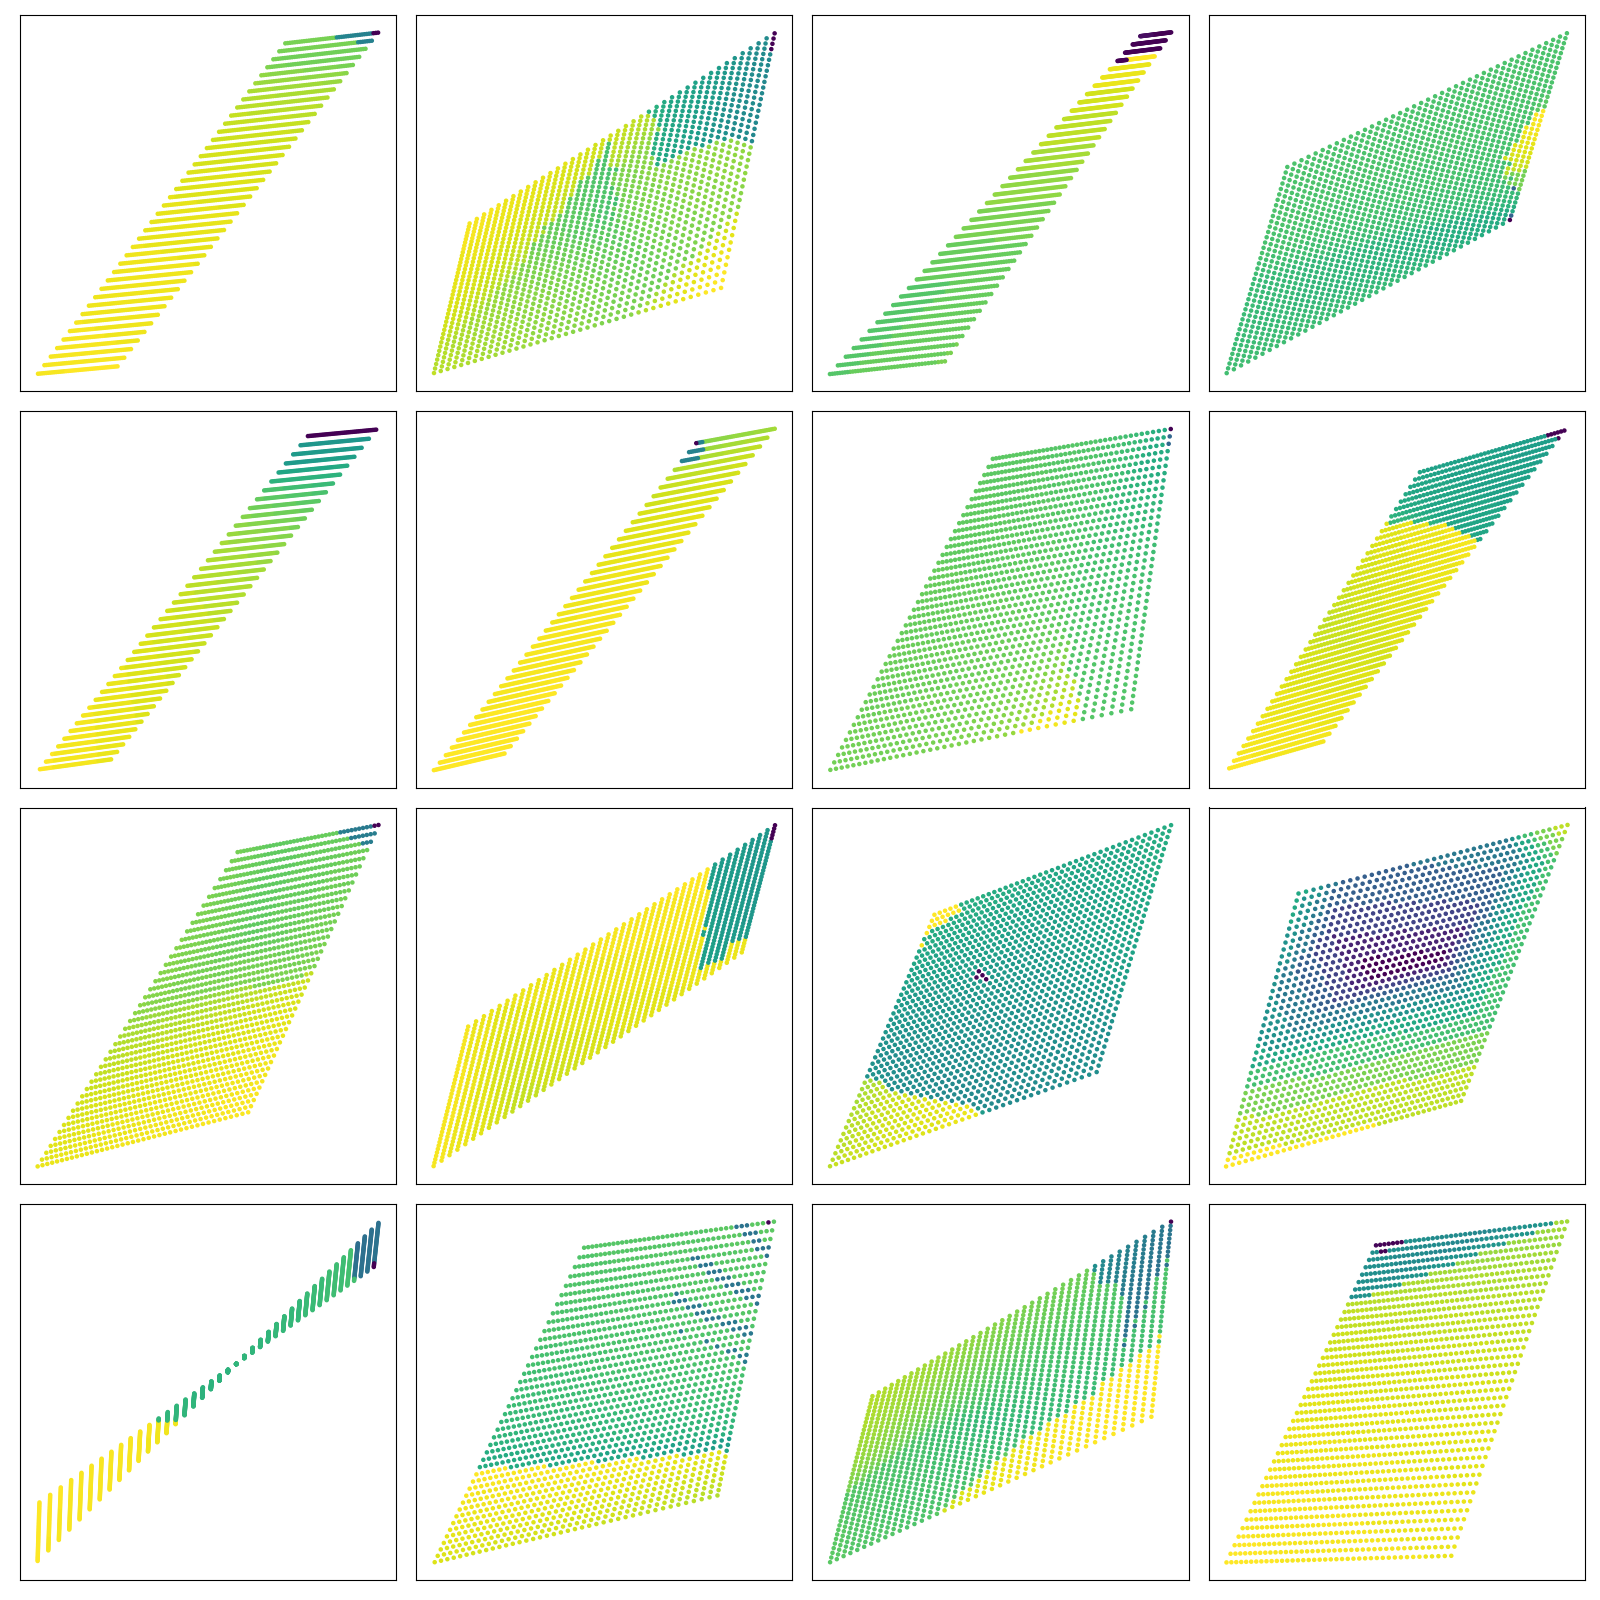
\includegraphics[width=1\textwidth,height=1\textheight]{../../pictures/figures/mvi-iterations.png}
\caption{Above you see: various MDPs where the value of each policy is colored
by the number of iterations it took to converge to the optimum policy. Yellow is many iterations, purple is few iterations.}
\end{figure}

\begin{itemize}
\tightlist
\item
  What are the best ways to travel through policy space? (lines of
  shortest distance?!)
\item
  How does this scale with \texttt{n\_actions} or \texttt{n\_states}??
\item
  Is there a way to use an interior search to give info about the
  exterior? (dual methods?!)
\item
  What if your evaluations are only \(\epsilon\)-accurate? How does that
  effect things?!?
\item
  how can we pick the topology for better dynamics!?
\end{itemize}



%  include iteration plots

The momentum polts tell us that if we want to bound the iteration complexity of GD plus momentum
then ...? We need a term that caputures the position / oscillation dynamics!?
% TODO want a better picture of the difference between these trajectories.


\subsection{Acceleration and parameterisation}

{\color{red}insert iteration complexity figures of different lrs with parameterisation.}

\cite{Arora2018} shows that overparameterisation yields acceleration. Consider
the dynamics of the parameter $w$, which we have overparameterised as $w_1 \cdot w_2$.


% Does it even make sense to do a first order approx when trying to reason about momentum?
% Momentum get interesting when considering non-first order factors?!?

We have implicit momentum from the parameterisation, and explicit momentum in the accelerated descent.


\begin{align}
m_{t+1} &= \gamma m_t + g_t \\
w_{t+1} &= w_t - \eta \cdot (1-\gamma) \cdot m_t
\end{align}

It is necessary to consider the trajectory to study momentum. It depends
on what has happened in the past. Can we construct a space of possible
trajectories? What properties do trajectories have? They are connected
by the update fn.

\section{Topology and dynamics}

What kinds of query and movement does our search space support?

If we parameterise our search space. We my have changed the topology of our search space.
Is it possible to arbitrarily change the topology? (probably?!?)

\textbf{Q:} How can we rationally pick the topology of our search space
to accelerate learning?

\begin{itemize}
\item
  A well connected space? For all possible policies, there exists
  \(\theta_1, \theta_2 \text{ s.t. } \parallel \theta_1- \theta_2\parallel_2\)
  is small. (but that doesnt necessarily help\ldots{} depends on the
  landscapce imposed by \(\nabla_{\theta} V\))
\item
  ???
\end{itemize}

See these gradient flows for example;

Pics?!?

Here are some examples \ldots{}???

\begin{figure}
\centering
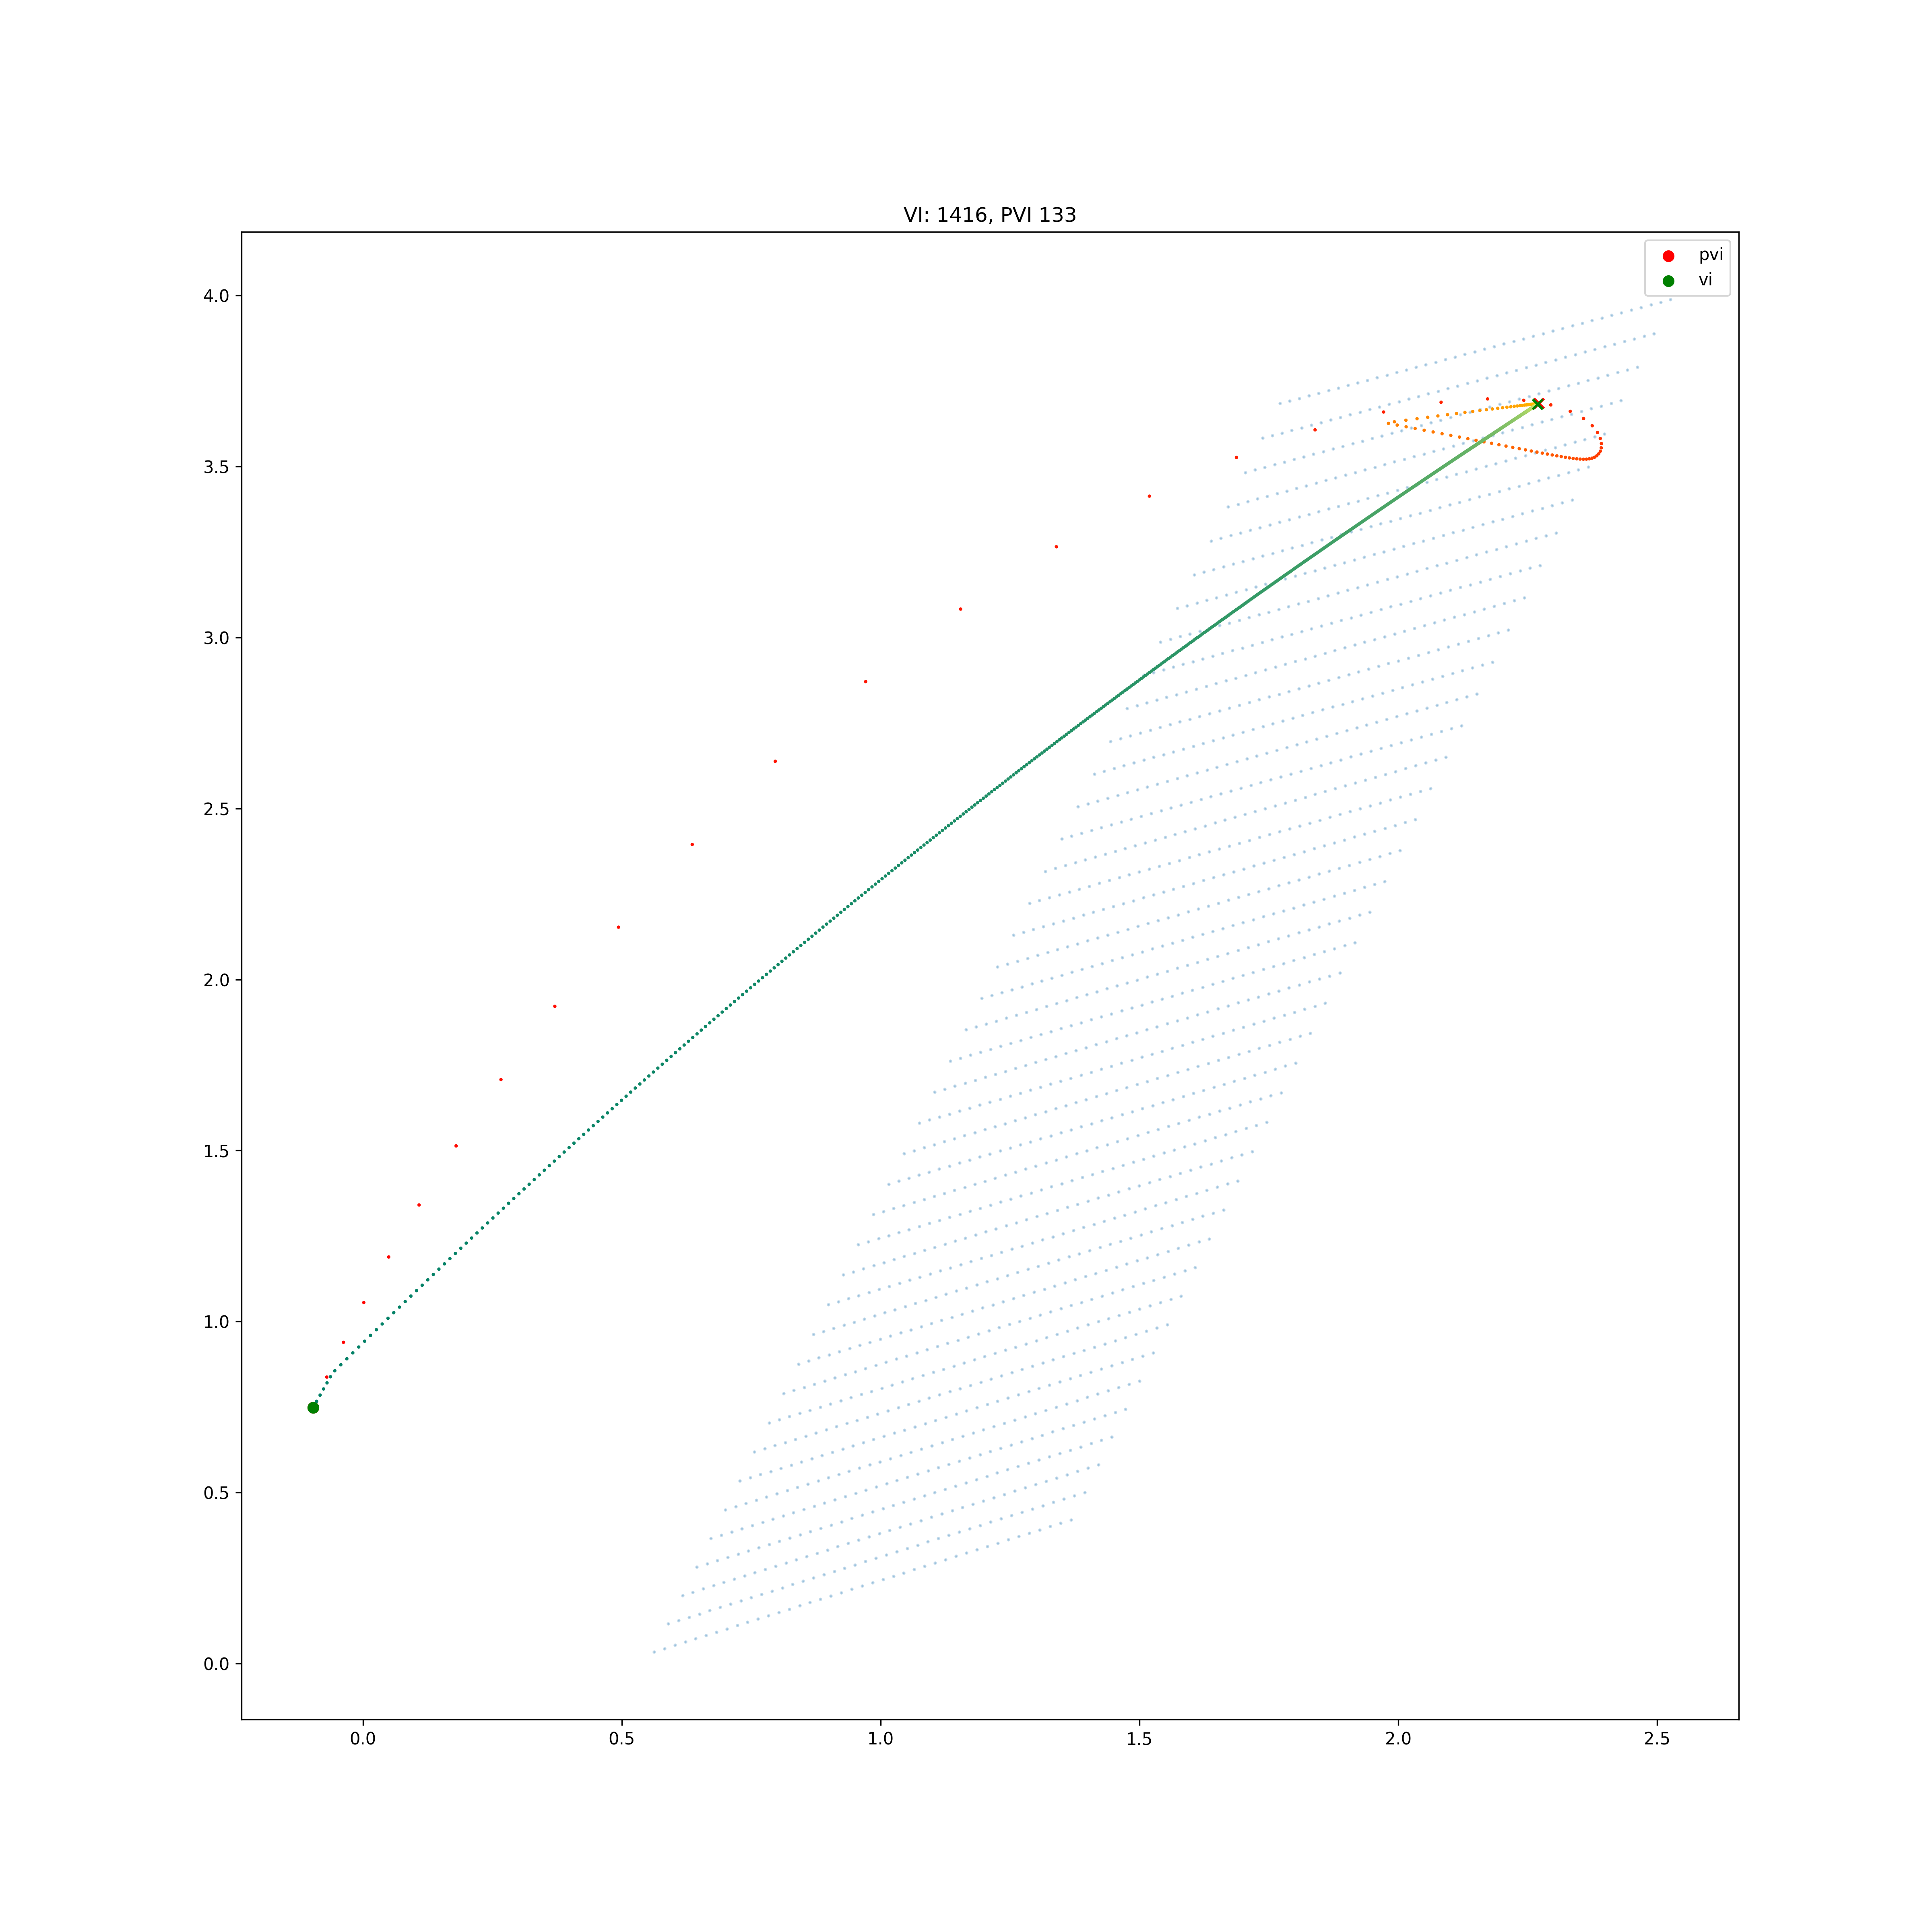
\includegraphics[width=0.5\textwidth,height=0.5\textheight]{../../pictures/figures/vi-vs-pvi.png}
\caption{The optimisation dynamics of value iteration versus parameterised value iteration.}
\end{figure}

\begin{figure}
\centering
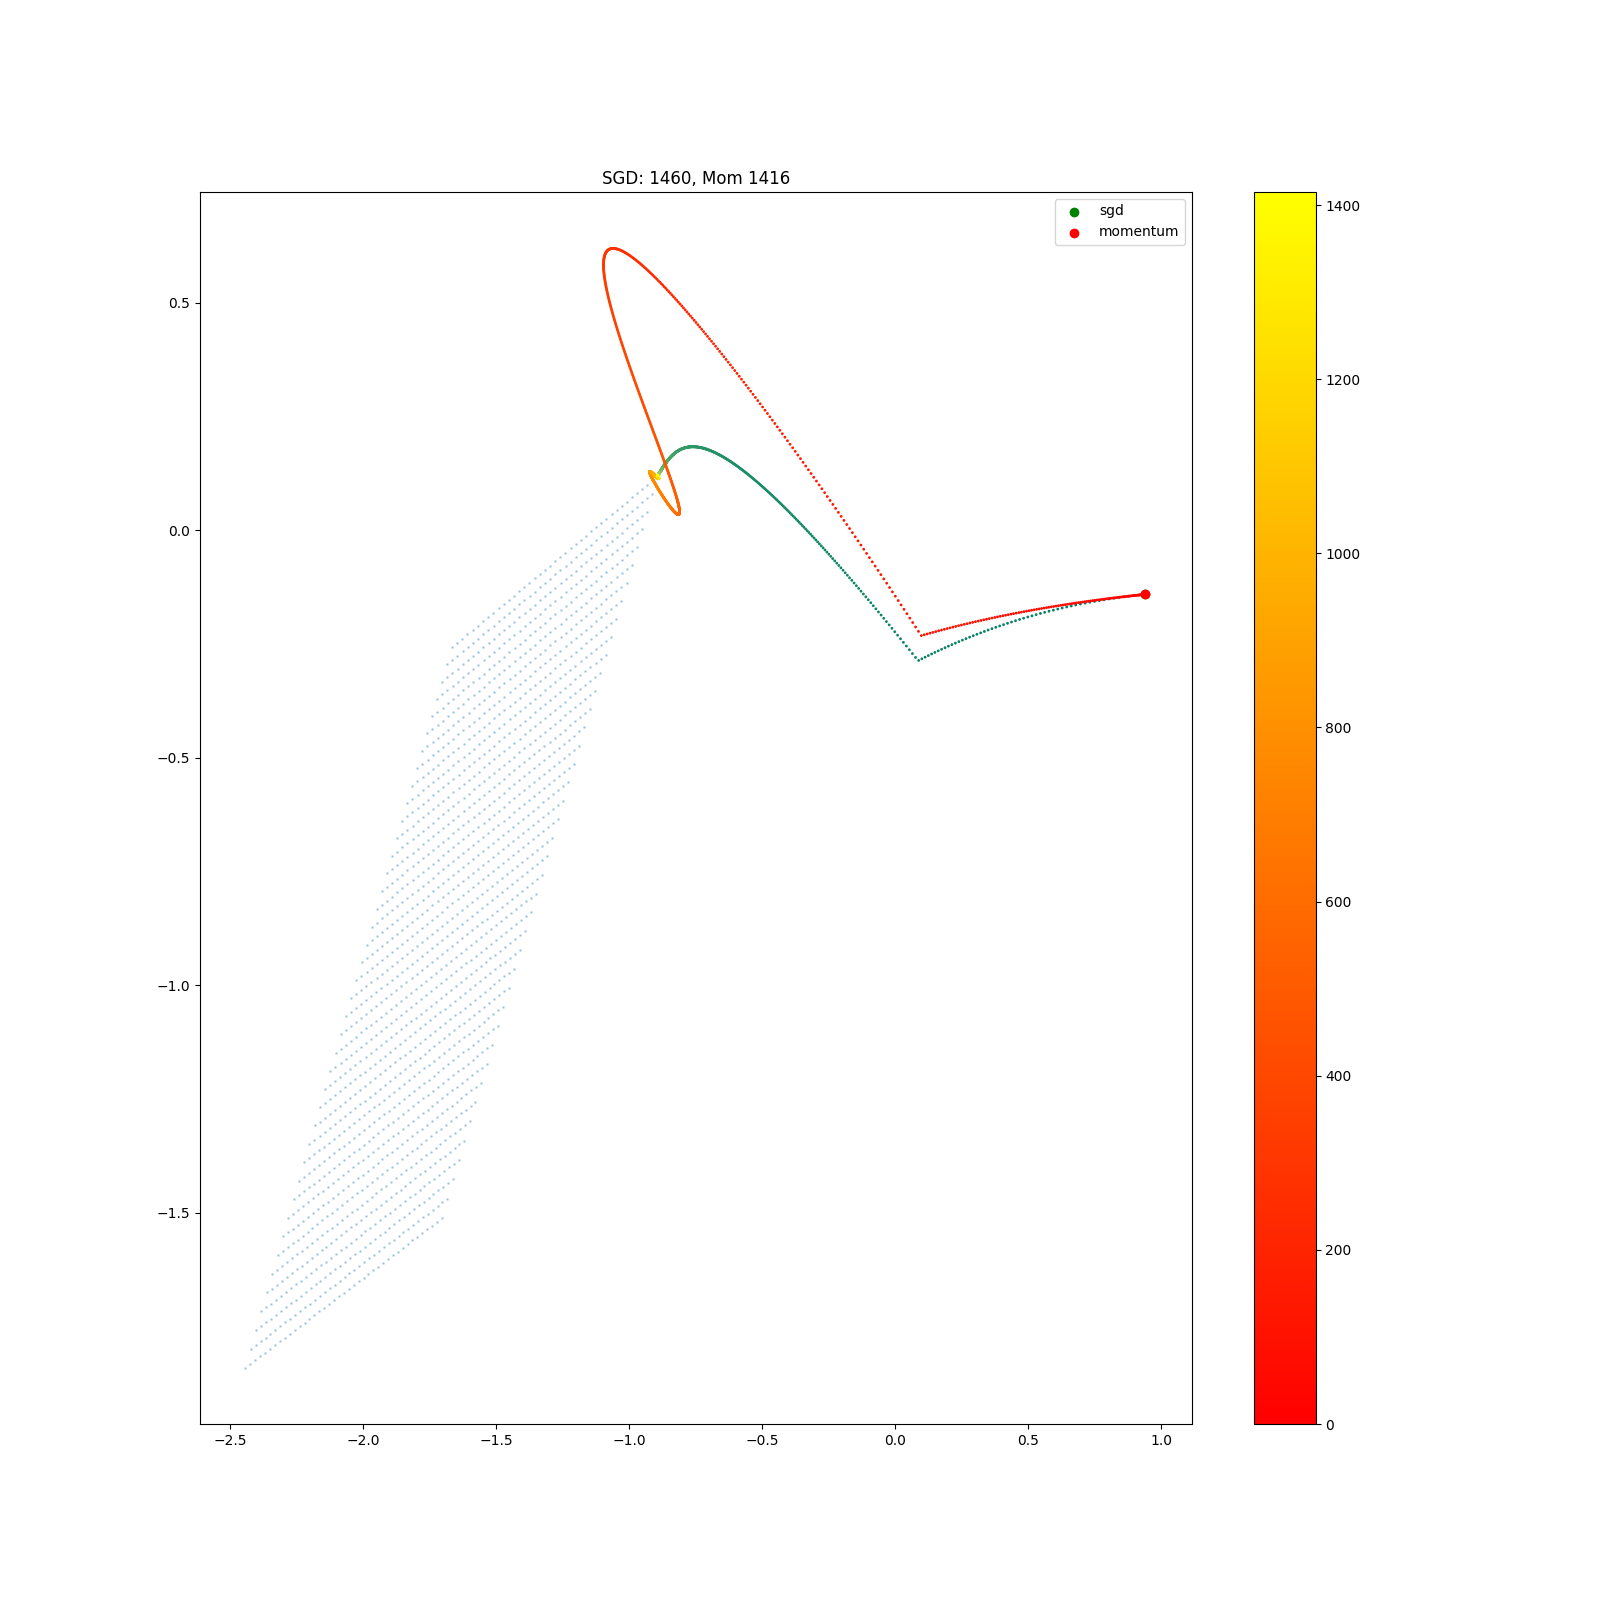
\includegraphics[width=0.5\textwidth,height=0.5\textheight]{../../pictures/figures/vi_sgd-vs-vi_mom.png}
\caption{The optimisation dynamics of value iteration versus value iteration with momentum.}
\end{figure}

If we overparameterise the search space, then we can move between solutions in new ways. We can `tunnel' from A to B, without crossing C.
%  insert pic / prove

Every point (in output space) is closer, when measured in the distance in parameter space needed to be traveled.
% insert pic / prove

\section{Notes}

When transforming between two spaces, how does the optimisation space
change? Does my abstraction make optimisation easier?


\section{Related work}

Recently there has been work investigating the properties of overparameterised search spaces.
Many \cite{Arora2018} (and others?!?!?) claim that overparameterisation yeilds acceleration, however,
their explanation of the acceleration is not entirely convincing. Bc...

How does momentum bias the kinds of solution that is converged to. (not really a question for RL?!)
Do we care aout the intermediate policies? In the synchronous setting no. In the asynchronous setting yes.
How does momentum bias trajectories? To cover more distance? To have more diversity?

Search spaces with alternative geometries.
Hyperbolic neural networks. https://arxiv.org/pdf/1805.09112.pdf


\section{Visualising higher dimensional MDPs}

So this value polytope works well for 2D. And possibly 3D. But,
"To deal with a 14-dimensional space, visualize a 3-D space and say 'fourteen' to yourself very loudly. Everyone does it." -- Geoff Hinton.

How to construct them?

Properties of the graphs / graph signals?


\subsection{Compressed sensing}

Related to !?!


\section{Conslusion}

So, we have seen, from our brief exploration of some properties of MDPs, that
there are some mysteries of interest to the ML community: the optimisation dynamics and generalisation of
parameterised function approximators.
There are unexplored types of solution strategy (???): model iteration. Which might be of interest to

So, while MDPs may be simple, we have yet to fully understand them or explore their ???.

Havent characterised their complexity?!? Sparse, ...

Hopefully we are now prepared to consider how abstraction can be used to improve the efficiency of RL for solving MDPs.
